\documentclass[12pt]{article}
% Эта строка — комментарий, она не будет показана в выходном файле
\usepackage{ucs}
\usepackage[warn]{mathtext}
\usepackage[utf8x]{inputenc} % Включаем поддержку UTF8
\usepackage[russian]{babel}  % Включаем пакет для поддержки русского языка
\usepackage{amsmath}
\usepackage{mathtools}
\usepackage{amssymb}
% \usepackage[dvips]{graphicx}
% \graphicspath{{noiseimages/}}
\usepackage[pdftex]{graphicx}


% Параметры страницы: 1см от правого края и 2см от остальных.


\hoffset=0mm
\voffset=0mm
\textwidth=180mm        % ширина текста
\oddsidemargin=-6.5mm   % левое поле 25.4 - 5.4 = 20 мм
\textheight=240mm       % высота текста 297 (A4) - 40
\topmargin=-15.4mm      % верхнее поле (10мм)
\headheight=5mm      % место для колонтитула
\headsep=5mm          % отступ после колонтитула
\footskip=8mm         % отступ до нижнего колонтитула

\begin{document}
	\author {Жарков Андрей 495}
	\title {Лабораторная работа 5.2 \\  Опыт Франка-Герца.}
    \maketitle{}
    
    \begin{center}
    	\textbf{\large Теоретические сведения}\\
    	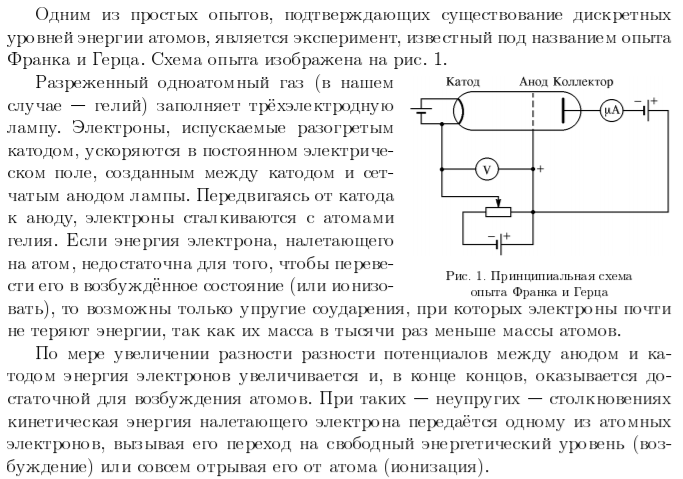
\includegraphics[width=14cm]{theory1.png}\\
    	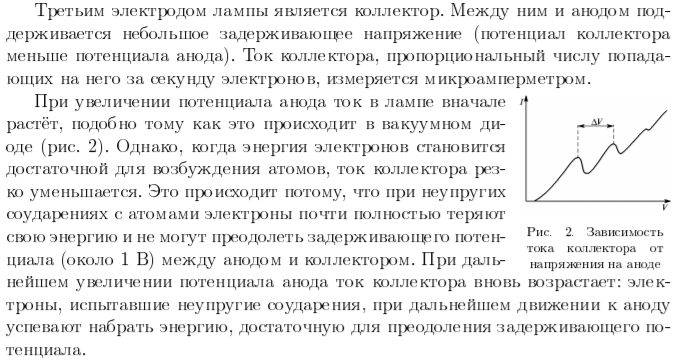
\includegraphics[width=14cm]{theory2.png}\\
    	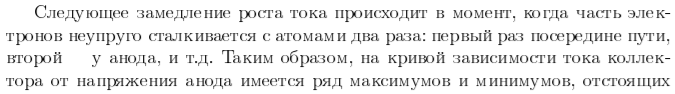
\includegraphics[width=16cm]{theory3.png}\\
    	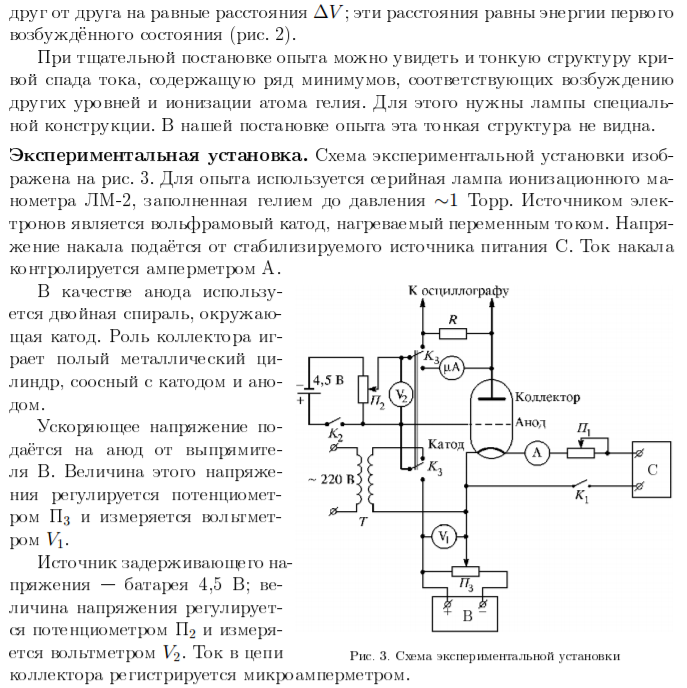
\includegraphics[width=16cm]{theory4.png}\\
    \end{center}
    
    \begin{center}
    	\textbf{\large Ход работы.}
    \end{center}
    
    1. Получим ВАХ $I_K = f(V_a))$ в динамическом режиме. Для этого сначала измерим при максимальном ускоряющем напряжении расстояния между максимумами и минимумами осциллограммы при различных значениях задерживающего напряжения.
    
    \begin{center}
    	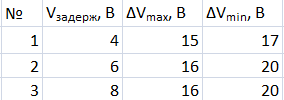
\includegraphics[width=6cm]{table1.png}
    \end{center}
    
    При измерениях $\sigma_{V_{max}} = \sigma_{V_{min}} = 0.5B$.
    
    Определим энергию возбуждения первого уровня атома гелия по формуле: $$E_1 = e\Delta U$$
    
    Ошибку оценим по формуле погрешности среднего арифметического: $$\sigma_{\Delta U} = \sqrt{\frac{1}{n(n-1)}\Sigma (\Delta U_i - \Delta U_{ср})^2}$$
    
    Итак, $E_1 = 17 \pm 2$ эВ.\\
    
    2. Теперь получим вольт-амперную характеристику в статическом режиме. Снимем завиимость коллекторного тока от анодного напряжения $I_K = f(V_a))$ для нескольких значений задерживающего напряжения. Результаты измерений приведены в таблице:
    
    \begin{center}
    	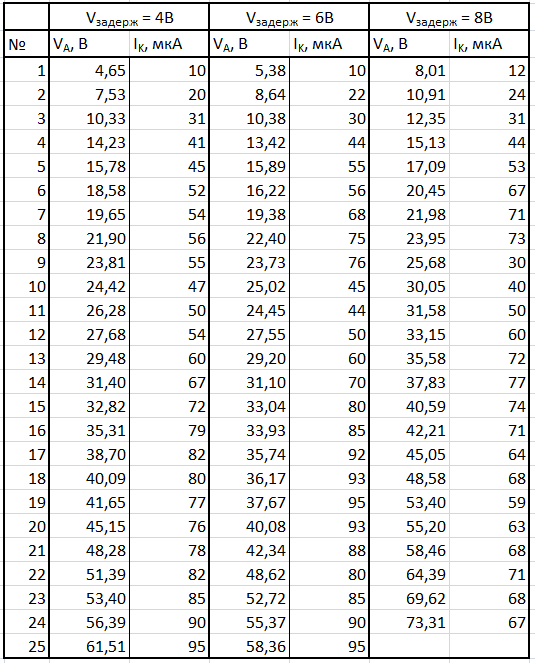
\includegraphics[width=13cm]{table2.png}
    \end{center}
    
    Построим графики для каждого значения задерживающего напряжения:
    
    \begin{center}
    	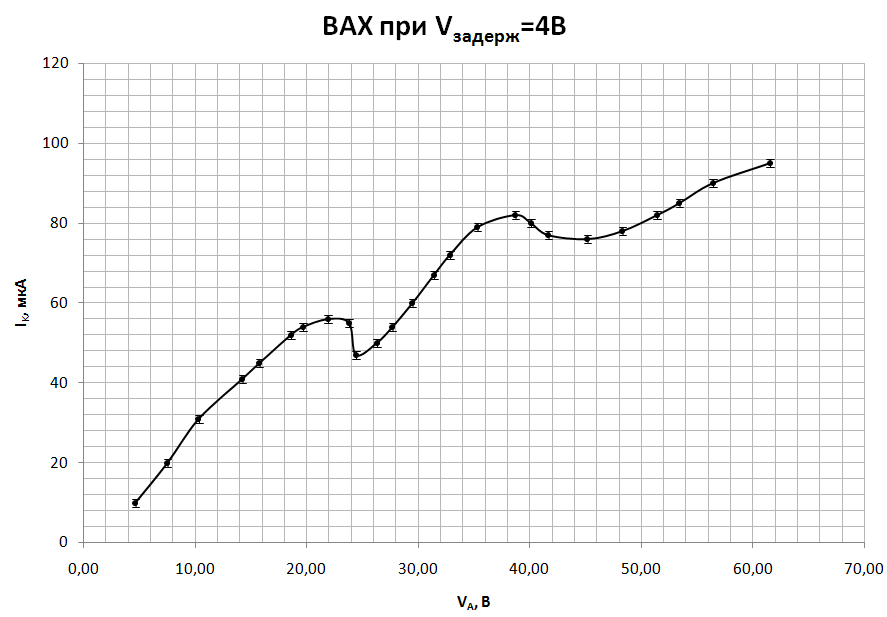
\includegraphics[width=15cm]{graph1.png}
    	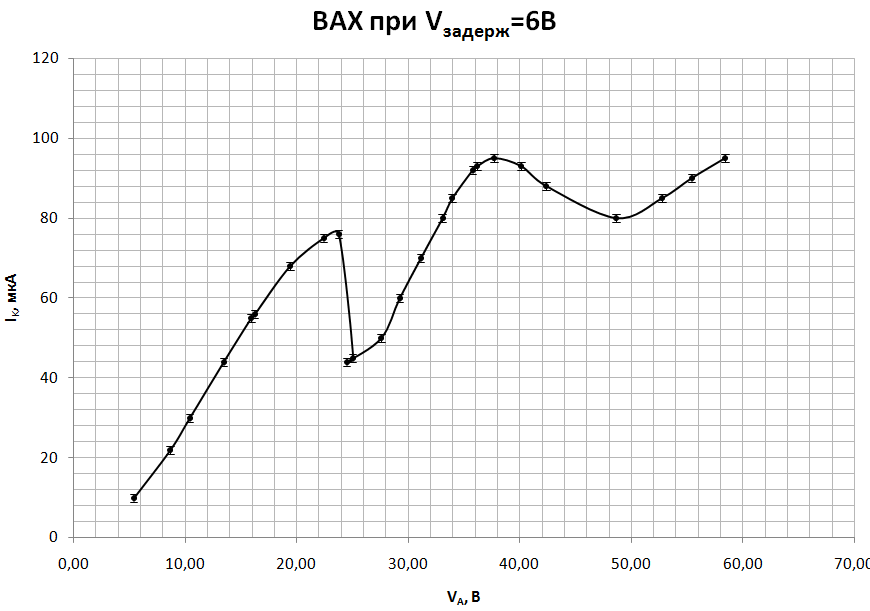
\includegraphics[width=15cm]{graph2.png}
    	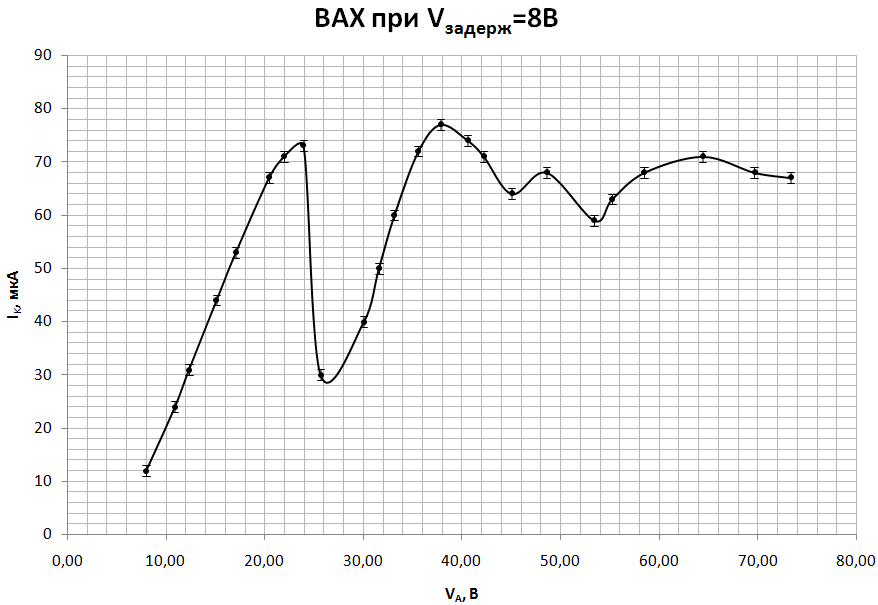
\includegraphics[width=15cm]{graph3.png}
    \end{center}
    
    Для каждого графика определим $\Delta U_{max}$ и, воспользовавшись формулой $E_1 = e\Delta U$ определим энергию возбуждения.
    
    При $V_{задерж} = 4В$ $E_1 = 18 \pm 1 эВ$
    
    При $V_{задерж} = 6В$ $E_1 = 18 \pm 1 эВ$
    
    При $V_{задерж} = 8В$ $E_1 = 16 \pm 1 эВ$
    
    Как видим, установленное на опыте значение энергии возбуждения первого уровня атома гелия несколько меньше табличного (табличное значение 19,8 эВ).
    
    Возможно, это связано с неидеальностью установки (например, гелий несколько разбавлен воздухом).
    
\end{document}